
Name  servers  are used  to  locate  objects  using a  human--readable
reference (their  name) rather than  a machine or network  address. If
objects providing  a certain service  are looked up using  the service
name, their  clients are  decoupled from the  actual locations  of the
objects that provide  this service.  The binding from  name to service
can be changed without the clients needing to know.

JacORB provides an implementation of the OMG's Interoperable Naming
Service (INS) which supports binding names to object references and to
lookup object references using these names.  It also allows clients to
easily convert names to strings and vice versa.  The JacORB name
service comprises two components: the name server program, and a set
of interfaces and classes used to access the service.


One word of caution about using JDK 1.2 with the JacORB naming
service: JDK 1.2 comes with a couple of outdated and apparently buggy
naming service classes that do not work properly with JacORB. To avoid
having these classes loaded and used inadvertently, please make sure
that you always use the {\tt NamingContextExt} interface rather than
the plain {\tt NamingContext} interface in your code. Otherwise, you
will see your application receive null pointer or other exceptions.

\section{Running the Name Server}

The JacORB  name server is a  process that needs to  be started before
the name service can be accessed by programs. Starting the name server
is done by typing on the command line either simply

\cmdline{ns [-Djacorb.naming.ior\_filename=<filename>] [-DOAPort=port] [-Djacorb.naming.time\_out=<timeout>]}

You can also start the Java interpreter explicitly by typing

\cmdline{jaco jacorb.naming.NameServer [-Djacorb.naming.ior\_filename=<filename>] [-DOAPort=port] [-Djacorb.naming.time\_out=<timeout>]}

In the example

\cmdline{ns -Djacorb.naming.ior\_filename=/home/me/public\_html/NS\_Ref}

we direct the name server process to write location information (its
own object reference) to the file {\tt /home/me/public\_html/NS\_Ref}.
A client--side ORB uses this file to locate the name server process.
The client--side ORB does not, however, need to be able to access the file through a
local or shared file system because  the file is read as a
 resource by using a URL pointing to it.  This implies that the
name server log file is accessible through a URL in the first place,
i.e., that you know of a web server in your domain which can answer
HTTP request to read the file.

The advantage of this approach is  that clients do not need to rely on
a hard--coded well known port  and that the name server is immediately
available world--wide  if the URL uses  HTTP. If you  want to restrict
name server visibility  to your domain (assuming that  the log file is
on a shared  file system accessible throughout your  domain) or you do
not have  access to a  web server, you  can use file URLs  rather than
HTTP URLs,  i.e. the URL pointing  to your name server  log file would
looks like

\noindent{\tt file:/home/brose/public\_html/NS\_Ref}

rather than

\noindent\verb+http://www.inf.fu-berlin.de/~brose/NS_Ref+

Specifying file URLs is also useful is clients and servers are run on
a single machine that may have no network connection at all. Please
note that the overhead of using HTTP is only incurred once --- when
the clients first locate the name server.  Subsequent requests will
use standard CORBA operation invocations which means they will be IIOP
requests (over TCP). In JacORB 1.4, the file name argument was made
optional because the JacORB 1.4 name server also answers requests that
are made using simplified corbaloc: URLs of the form {\tt
  corbaloc::ip-address:port/NameService}. This means that all you need
to know to construct an object reference to your name service is the
IP address of the machine and the port number  the server process is
listening on (the one specified using {\tt -DOAPort=<port>}).

The name server stores its  internal state, i.e., the name bindings in
its context,  in files  in the current  directory unless  the property
{\tt jacorb.naming.db\_dir} is set to a different directory name. This
saving is done  when the server goes down  regularly, i.e. killing the
server  with CTRL-C  will result  in loss  of data.   The  server will
restore state from its files if any files exist and are non--empty.

The second  parameter is a port number on which you want the name
service to listen for incoming requests. If this parameter is not
set, the name server will come up on the first free port it is
provided with by the operating system. The port number can also be set
using specific properties in the properties file, but the -DOAPort=<port> switch
was added merely for convenience.

The last  parameter is a time--out  value in msecs. If  this value is
set, the name server will shut down after the specified amount of time
and save  its state. This is  useful if the name  server is registered
with  the  Implementation Repository  and  can  thus  be restarted  on
demand.

\subsection*{Configuring a Default Context}

Configuring a naming context (i.e. a name server) as the ORB's default
or root context is done by  simply writing the URL that points to this
server's    bootstrap    file   to    the    properties   file    {\tt
.jacorb\_properties}.  Alternatively,  you can  set this file  name in
the property {\tt ORBInitRef.NameService} either on the command line or
within the application  as described in \ref{Sec_installation}.  After
the default  context has thus  been configured, all operations  on the
NamingContextExt  object  that  was   retrieved  by  a  call  to  {\tt
orb.resolve\_initial\_references("NameService")}   will  go   to  that
server  ---  provided  it's  running  or  can  be  started  using  the
Implementation Repository.

\section{Accessing the Name Service}

The  JacORB name  service is accessed using  the standard  CORBA
defined  interface:

\small{
\begin{verbatim}
   // get a reference to the naming service
   ORB orb = ORB.init(args, null);
   org.omg.CORBA.Object o = orb.resolve_initial_references("NameService")
   NamingContextExt nc = NamingContextExtHelper.narrow( o );

   // look up an object
   server s = serverHelper.narrow( nc.resolve(nc.to_name("server.service")) );
\end{verbatim}
}

Before an object  can be looked up, you need a  reference to the ORB's
name service. The standard way  of obtaining this reference is to call
{\tt orb.resolve\_initial\_\-referen\-ces("Name\-Service")}.  In calls using
the  standard,  extended  name  service interface,  object  names  are
represented as  arrays of {\tt NameComponent}s rather  than as strings
in  order to  allow  for  structured names.   Therefore,  you have  to
construct such an  array and specify that the  name's name is "server"
and    that    it    is    of   kind    ``service''    (rather    than
``context'').    Alternatively,    you    can   convert    a    string
``server.service''  to a  name by  calling the  {\tt NamingContextExt}
interface's {\tt to\_name()} operation, as shown above.

Now,  we can  look up  the object  by calling  {\tt resolve()}  on the
naming context, supplying the array as an argument.

\section{Constructing Hierarchies of Name Spaces}

Like directories in a file system, name spaces or contexts can contain
other contexts  to allow hierarchical structuring instead  of a simple
flat name  space. The  components of a  structured name for  an object
thus  form a path  of names,  with the  innermost name  space directly
containing the  name binding for the  object. This can  very easily be
done using {\tt NameManager} but can also be explicitly coded.

A new naming context within  an enclosing context can be created using
either   {\tt  new\_context()}   or  {\tt   bind\_new\_context()}.  The
following code snippet requests a naming context to create an inner or
subcontext using a given name and return a reference to it:
\small{\begin{verbatim}
   // get a reference to the naming service
   ORB orb = ORB.init();
   org.omg.CORBA.Object o =
      orb.resolve_initial_references("NameService");
   NamingContextExt rootContext =
      NamingContextExtHelper.narrow( o );

   // look up an object
   NameComponent[] name = new NameComponent[1];
   name[0] = new NameComponent("sub","context");
   NamingContextExt subContext =
     NamingContextExtHelper.narrow( rootContext.bind_new_context( name ));
\end{verbatim}}

Please  note   that  the  JacORB  naming  service   always  uses  {\tt
NamingContextExt} objects internally,  even if the operation signature
indicates {\tt  NamingContext} objects.  This is  necessary because of
the limitations  with JDK  1.2 as explained  at the beginning  of this
section.

\section{NameManager --- A simple GUI front-end to the Naming Service}

The graphical front-end to the name service can be started by calling

\cmdline{nmg}

The GUI front-end will simply look up the default context and display
its contents. Figure \ref{fig:nameManager} gives a screen shot.

\bigskip
\begin{figure}[htb]
  \begin{center}
    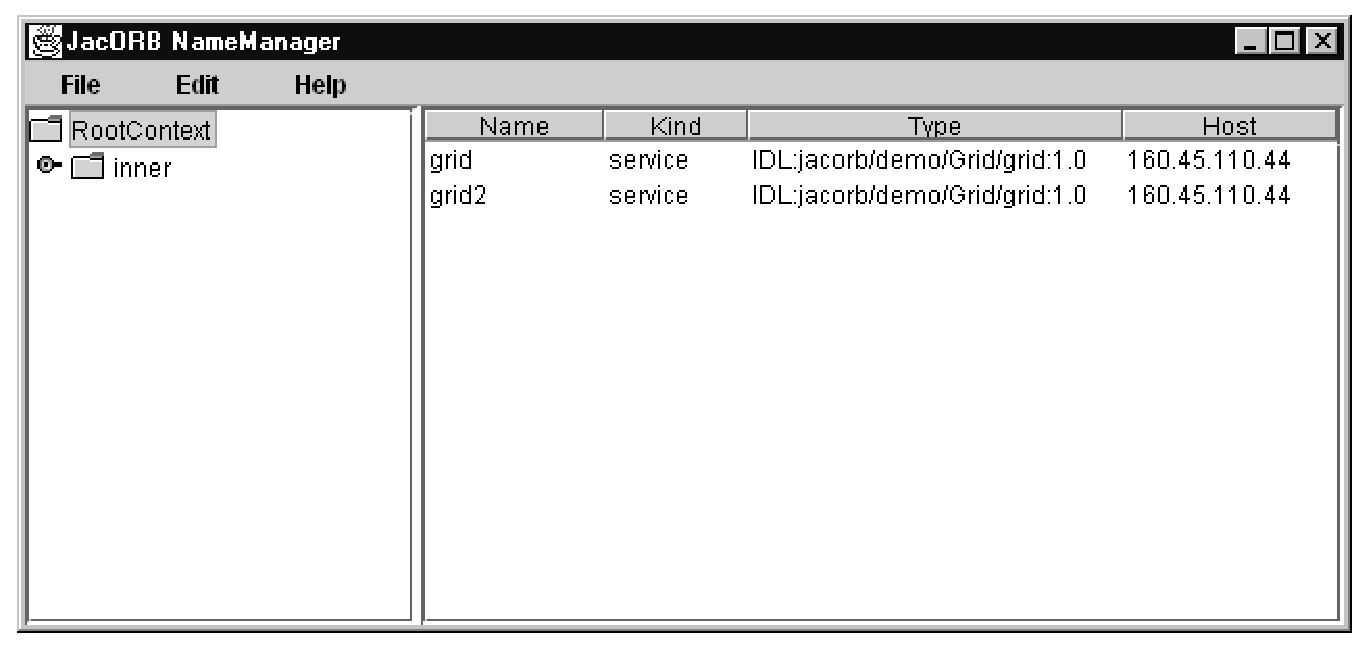
\includegraphics[width=10cm]{Naming/Nmgr1}
  \end{center}
\caption{NameManager Screenshot}
\label{fig:nameManager}
\end{figure}

NameManager has menus that let you bind and unbind names, and create
or delete naming contexts within the root context. Creating a nested
name space, e.g., can be done by selecting the {\tt RootContext} and
bringing up a context by clicking the right mouse button.  After
selecting ``new context'' from that menu, you will be prompted to
enter a name for the new, nested context.


%%% Local Variables: 
%%% mode: latex
%%% TeX-master: "../ProgrammingGuide"
%%% End: 
